\begin{figure}[H]
  \begin{center}
    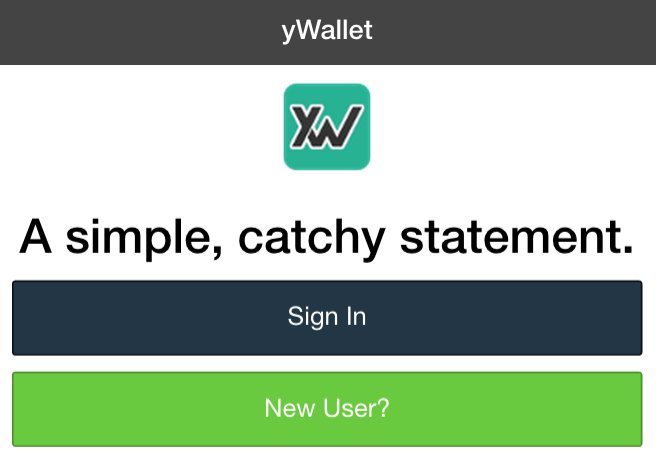
\includegraphics[width=0.5
    \textwidth]{authentication/init.png}
  \end{center}
  \caption{Autenticação}
  \label{fig:1}
\end{figure}

No ecrã de autenticação, é apresentada ao utilizador a possibilidade de registo e de \textit{login} na aplicação.

\subsection{Registo}
  \begin{figure}[H]
    \begin{center}
      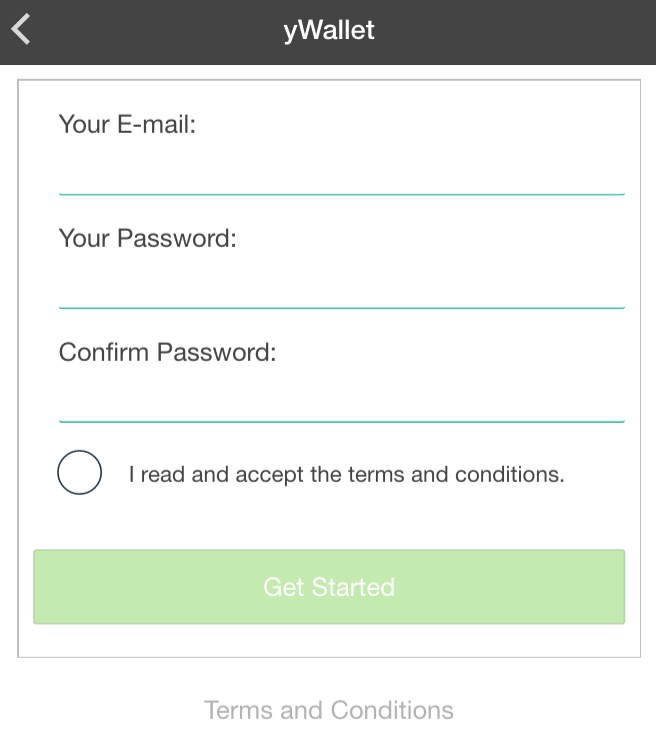
\includegraphics[width=0.5
      \textwidth]{authentication/register.png}
    \end{center}
    \caption{Registo}
    \label{fig:1_1}
  \end{figure}

Para utilizar a aplicação é necessário o utilizador já ter uma conta  \textit{Coinbase}. Caso não tenha existe a possibilidade de criar no processo de registo. Para criar o registo apenas é necessário o email do utilizador e uma \textit{password}. Apenas os pais (\textit{managers}) necessitam de criar conta. Os filhos são adicionados pelos pais. (ver secção \ref{sec:conf}).

\subsection{Login}
  \begin{figure}[H]
    \begin{center}
      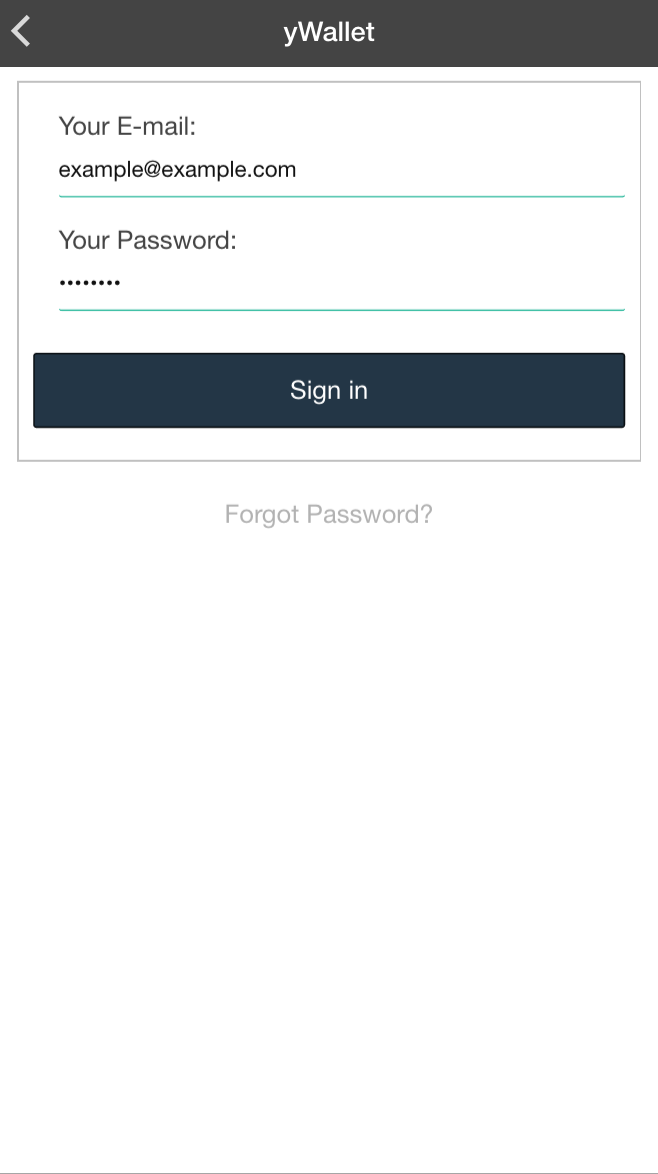
\includegraphics[width=0.5
      \textwidth]{authentication/login.png}
    \end{center}
    \caption{Login}
    \label{fig:1_2}
  \end{figure}

A Figura \ref{fig:1_2} apresenta o ecrã de \textit{login} na aplicação.

\subsection{Recuperar a \textit{Password}}
  \begin{figure}[H]
    \begin{center}
      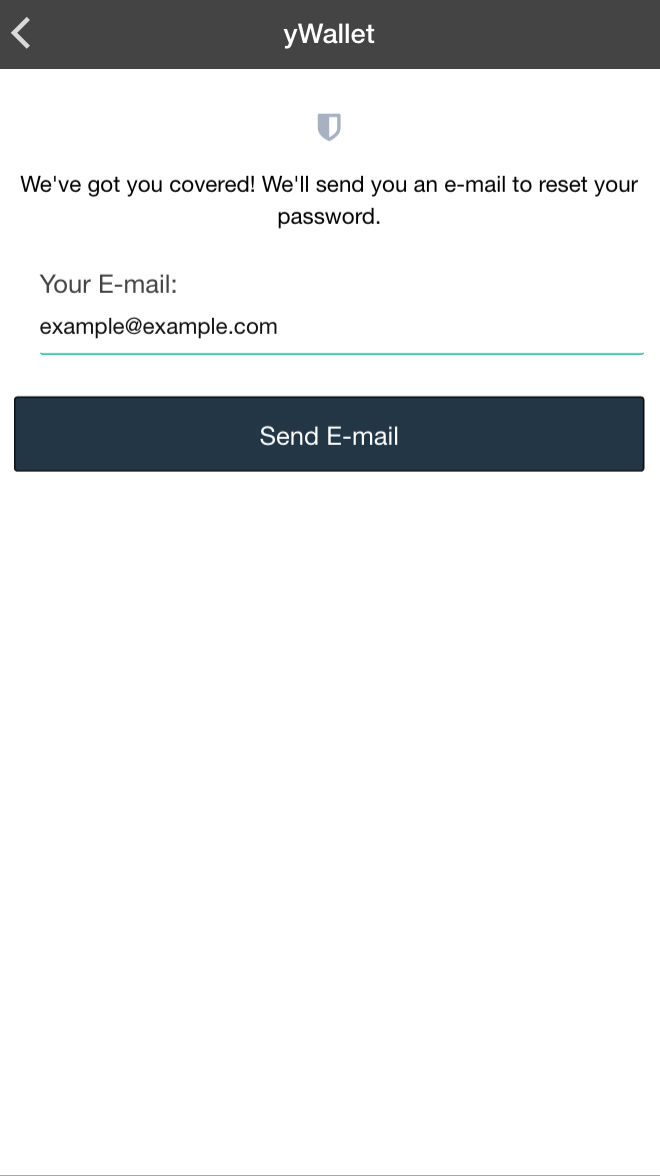
\includegraphics[width=0.5
      \textwidth]{authentication/forget.png}
    \end{center}
    \caption{Recuperar Password}
    \label{fig:1_3}
  \end{figure}

Caso o utilizador não se lembre da \textit{password} é possível recuperar utilizando a opção \textit{Forgot Password?} do ecrã de \textit{login} (Figura \ref{fig:1_2}). O ecrã de recuperação da \textit{password} é apresentado na Figura \ref{fig:1_3}.